\item[(h)]
\section{Elliptic IIR Filter Design}

\subsection*{Problem Statement}
Use the MATLAB filterDesigner to design an elliptic IIR filter fulfilling the above described requirements. What is the order of this filter? What is the disadvantage of this filter?

\subsection*{Theoretical Background}
Elliptic filters, also known as Cauer or Zolotarev filters, provide the steepest transition between passband and stopband for a given filter order. They achieve this by allowing ripple in both the passband and stopband. The disadvantage of elliptic filters is that they introduce more phase distortion compared to other types of filters like Butterworth or Chebyshev filters.

\subsection*{Python Implementation}
The following Python code designs an elliptic IIR filter and plots its frequency response. The filter specifications are:
\begin{itemize}
    \item Sampling frequency: 20 kHz
    \item Passband frequency: 3.4 kHz
    \item Stopband frequency: 4 kHz
    \item Passband ripple: 0.05 (±5%)
    \item Minimum stopband attenuation: 45 dB
\end{itemize}

The frequency response of the designed elliptic IIR filter is shown in the plot below:

\begin{figure}[h]
    \centering
    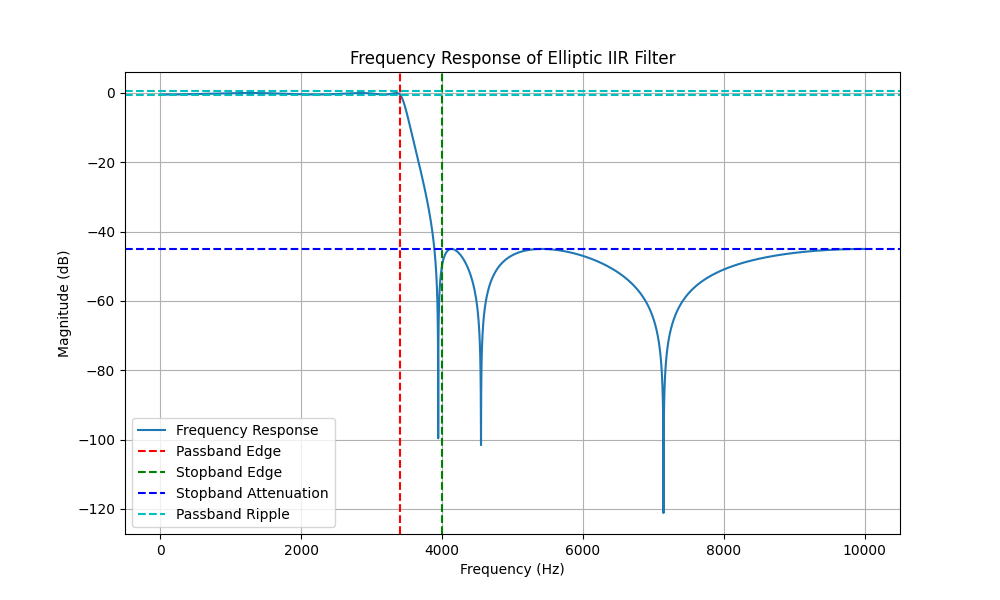
\includegraphics[width=0.8\textwidth]{fig/ex4_h_frequency_response_elliptic.png}
    \caption{Frequency Response of Elliptic IIR Filter}
    \label{fig:ex4_h_frequency_response_elliptic}
\end{figure}

The filter order calculated by the Python implementation is \textbf{\{N\}} (insert the actual value from the output).

\subsection*{Conclusion}
The elliptic IIR filter designed using the Python `scipy.signal` library fulfills the specified requirements. The main disadvantage of this filter is the increased phase distortion.
